% concatenated from main.tex, cas.tex
\documentclass[11pt]{article}
\usepackage{amsmath}
\usepackage{amssymb}
\usepackage{amsthm}
\usepackage{geometry}
\usepackage{hyperref}
\usepackage{listings}
\usepackage{xcolor}
\usepackage{enumitem}
\usepackage[T1]{fontenc}
\usepackage{comment}
\usepackage{tikz,array}
\usepackage{indentfirst}
\usepackage{subcaption}

\geometry{a4paper, margin=1in}


% Define colors for the listings
\definecolor{codegreen}{rgb}{0,0.6,0}
\definecolor{codegray}{rgb}{0.5,0.5,0.5}
\definecolor{codepurple}{rgb}{0.58,0,0.82}
\definecolor{backcolour}{rgb}{0.95,0.95,0.92}

% Listings configuration for C++
\lstdefinestyle{cppstyle}{
    backgroundcolor=\color{backcolour},
    commentstyle=\color{codegreen},
    keywordstyle=\color{blue},
    numberstyle=\tiny\color{codegray},
    stringstyle=\color{codepurple},
    basicstyle=\ttfamily\footnotesize,
    breakatwhitespace=false,
    breaklines=true,
    captionpos=b,
    keepspaces=true,
    numbers=left,
    numbersep=5pt,
    showspaces=false,
    showstringspaces=false,
    showtabs=false,
    tabsize=4
}

\lstset{style=cppstyle}

\title{Distribution of independent sets in perfect $r$-ary trees}
\author{Daniel I\v{l}kovi\v{c}\thanks{Institute of Mathematics, Leipzig University, Augustusplatz 10, 04109 Leipzig, Germany. Mathematics Institute, University of Warwick, Coventry CV4 7AL, UK. \url{daniel.ilkovic@warwick.ac.uk}. Supported by the Alexander von Humboldt Foundation in the framework of the Alexander von Humboldt Professorship of Daniel Krá\v{l} endowed by the Federal Ministry of Education and Research.} \and Jun Yan\thanks{Mathematical Institute, University of Oxford, Oxford OX2 6GG, UK. Email: \url{jun.yan@maths.ox.ac.uk}. Supported by
ERC Advanced Grant 883810.}}

\newtheorem{theorem}{Theorem}[section]
\newtheorem{lemma}[theorem]{Lemma}
\newtheorem{conjecture}[theorem]{Conjecture}
%\newtheorem{definition}[theorem]{Definition}
\newtheorem{corollary}[theorem]{Corollary}
\newtheorem{question}[theorem]{Question}

\theoremstyle{definition}
\newtheorem{definition}[theorem]{Definition}

\newcommand{\cI}{\mathcal{I}}
\DeclareMathOperator{\cas}{CAS}

\newcounter{propcounter}

\begin{document}
\maketitle

\begin{abstract}
%A subset of vertices in a graph is an independent set if no two vertices within are adjacent. 
Given a graph $G$, the family of all independent sets of size $k$ containing a fixed vertex $v$ is called a star with centre $v$, and is denoted by $\cI_G^k(v)$. Motivated by a generalisation of the Erd\H{o}s-Ko-Rado Theorem to the setting of independent sets in graphs, Hurlbert and Kamat conjectured that for every tree $T$ and every $k$, the maximum of $|\cI_T^k(v)|$ can always be attained by a leaf of $T$. While this conjecture turns out to be false in general, it is known to hold for specific families of trees like spiders and caterpillars. In this paper, we prove that this conjecture holds for a new family of trees, the perfect $r$-ary trees, by constructing injections from stars centred at arbitrary vertices to stars centred at leaves. We also show that the analogous property holds for every forest $\mathcal{T}$ that is the disjoint union of perfect trees with possibly varying sizes and arities, and determine the leaf that maximises $|\cI_{\mathcal{T}}^k(v)|$. 

%We provide a direct, constructive proof that perfect binary trees satisfy this property. The proof relies on defining explicit injective mappings between the family of independent sets of size $k$ containing an internal vertex $v$ and the family of independent sets of the same size containing a leaf $l$. We construct two distinct algorithmic mappings, tailored to the parity of the distance between $v$ and $l$, utilizing techniques such as synchronised traversals and iterative path shifting.
\end{abstract}

\section{Introduction}
A family $\mathcal{F}$ of sets is called \textit{intersecting} if any $A,B\in\mathcal{F}$ satisfies $A\cap B\not=\varnothing$. The well-known Erd\H os-Ko-Rado Theorem~\cite{EKR}, published in 1961, states that if $n\geq2k$ and $\mathcal{F}$ is an intersecting family of subsets of $[n]$ of size $k$, then $|\mathcal{F}|\leq\binom{n-1}{k-1}$. Moreover, if $n>2k$, then equality holds if and only if $\mathcal{F}=\{A:i\in A, |A|=k\}$ for some $i\in[n]$. Since then, there have been many generalisations and variants of the Erd\H os-Ko-Rado Theorem in the literature. In this paper, we focus on a generalisation to the following setting of independent sets in graphs proposed by Holroyd, Spencer, and Talbot~\cite{HST,HT} in 2005. 

\begin{definition}
Let $G=(V(G), E(G))$ be a graph, let $v\in V(G)$, and let $k$ be an integer.  
\begin{itemize}
    \item A subset $I \subseteq V(G)$ is an \emph{independent set} in $G$ if $uw \notin E(G)$ for all $u, w \in I$. 
    \item The family of all independent sets of size $k$ in $G$ is denoted by $\mathcal{I}_{G}^{k}$.
    \item The family $\{A\in\mathcal{I}_{G}^{k}:v\in A\}$ of all independent sets of size $k$ in $G$ containing $v$ is denoted by $\mathcal{I}_{G}^{k}(v)$. Each family of the form $\cI_G^k(v)$ is called a \emph{star}, and $v$ is called its \emph{star centre}.
\end{itemize}
\end{definition}
Note that every star $\cI^k_G(v)$ is an intersecting family in $\cI^k_G$ by definition.

\begin{definition}
Let $G$ be a graph and let $k$ be an integer.
\begin{itemize}
    \item $G$ is \textit{$k$-EKR} if no intersecting family of sets in $\cI_G^k$ is larger than the largest star in $\cI_G^k$.
    \item $G$ is \textit{strictly $k$-EKR} if every intersecting family of sets in $\cI_G^k$ of maximum size is a star. 
\end{itemize}
\end{definition}
Observe that using this language, the Erd\H os-Ko-Rado Theorem can be restated as saying the empty graph on $n$ vertices is $k$-EKR if $n\geq 2k$, and strictly $k$-EKR if $n>2k$. 

Several families of graphs have been shown to be $k$-EKR for suitable values of $k$. These include powers of cycles~\cite{T}, powers of paths~\cite{HST}, and certain graphs with an isolated vertex~\cite{BH,HST,HK}. A major outstanding conjecture due to Holroyd and Talbot~\cite{HT} states that if $\mu(G)$ is the minimum size of a maximal independent set in $G$, then $G$ is $k$-EKR if $k\leq\mu(G)/2$, and strictly so if $k<\mu(G)/2$. Many positive results in this direction proceed by induction and use a shifting/compression proof technique involving the deletion of edges and vertices. The presence of an isolated vertex $x$ in $G$ is very useful as it is not affected by the deletion process, and due to the easy observation that for every $k$, the maximum of $|\cI_G^k(v)|$ can always be attained by $x$.

%The study of star centres in graphs is significantly motivated by their relation to Erd\H{o}s-Ko-Rado (EKR) type problems. A graph $G$ is said to be $k$-EKR if the largest intersecting family of independent sets in $\mathcal{I}_{G}^{k}$ is a star. Identifying the centre of the largest star is often a crucial step in verifying the EKR property.

%Investigating where independent sets tend to localise in graphs (with early related inquiries appearing in~\cite{LM}), Hurlbert and Kamat focused on trees and proposed the following conjecture~\cite{HK}:

For a graph $G$ without an isolated vertex, finding the centre of a star of maximum size is no longer trivial, and it seems difficult in general to prove that $G$ is $k$-EKR without knowing which star has maximum size. Motivated by this, Hurlbert and Kamat~\cite{HK} proposed to study the intermediate problem of determining which vertex $v\in V(G)$ maximises $|\cI^k_G(v)|$. In particular, they considered the case when $G$ is a tree, and conjectured that there is always a maximum-sized star centred at a leaf. 
\begin{conjecture}[\cite{HK}]\label{conj:HK}
For any $k\ge1$ and any tree $T$, there exists a leaf $\ell$ of $T$ such that $|\mathcal{I}_{T}^{k}(v)|\le|\mathcal{I}_{T}^{k}(\ell)|$ for every $v\in V(T)$.
\end{conjecture}

Hurlbert and Kamat proved this conjecture for $k\le4$~\cite{HK}. However, independent work of Baber~\cite{Baber} and Borg~\cite{Borg} produced counterexamples disproving Conjecture~\ref{conj:HK} for every $k\geq5$. Feghali, Johnson, and Thomas~\cite{FJT} produced further counterexamples showing that maximum-sized stars can be centred on a vertex with arbitrarily large degree and arbitrarily far away from any leaves in $T$, which disprove Conjecture~\ref{conj:HK} in a very strong sense. 

Even though Conjecture~\ref{conj:HK} is now disproved, it remains interesting to determine which trees satisfy the condition in Conjecture~\ref{conj:HK}. We use the following terminology introduced by Estrugo and Pastine in~\cite{EP}.
\begin{definition}
Let $T$ be a tree and let $k\geq1$ be an integer. 
\begin{itemize}
    \item $T$ is \textit{$k$-HK} if there exists a leaf $\ell$ of $T$ such that $|\mathcal{I}_{T}^{k}(v)|\le|\mathcal{I}_{T}^{k}(\ell)|$ for each $v\in V(T)$.
    \item $T$ is \textit{HK} if it is $k$-HK for every $k\geq1$.
\end{itemize}
\end{definition}
Two families of trees known to be HK are spiders~\cite{HK2} and caterpillars~\cite{EP}. We refer interested readers to a detailed survey~\cite{H} by Hurlbert of other results on graphs with EKR-type and/or HK-type properties.


%We say that a graph $G$ satisfies the \emph{HK property} if it satisfies Conjecture~\ref{conj:HK}. Despite the failure of the general conjecture, several classes of trees, such as spiders~\cite{HK} and caterpillars~\cite{EP}, have been shown to satisfy the HK property. The study of independent set distributions and related combinatorial structures remains an active area of research~\cite{JP}.

%\textbf{Our Contribution.} In this paper, we investigate the highly symmetric structure of perfect binary trees and prove that they satisfy the HK property. We provide a direct combinatorial proof based on explicit injective mappings. We construct algorithms that transform an independent set of size $k$ containing an internal vertex $v$ into a unique independent set of the same size containing a leaf $l$. This constructive approach leverages the recursive structure of perfect binary trees and involves two distinct strategies, depending on the parity of the distance between $v$ and $l$.

The main result of this paper, Theorem~\ref{thm:main}, shows that the perfect $r$-ary trees are HK. For every integer $r\geq2$, a \textit{perfect $r$-ary tree} with $h$ \textit{levels} is the unique rooted plane tree $T$ that has exactly $r^{h-1}$ leaves, all at distance $h-1$ away from the root, and whose non-leaf vertices all have exactly $r$ children. The \textit{arity} of a perfect $r$-ary tree is $r$. A \textit{perfect tree} is a perfect $r$-ary tree for some $r\geq2$. The $r=2$ case of Theorem~\ref{thm:main} answers a question of Hurlbert~\cite{H}. 

\begin{theorem}\label{thm:main}
Let $T$ be a perfect $r$-ary tree. For any integer $k \geq 1$, any vertex $v \in V(T)$, and any leaf $\ell \in V(T)$, we have $|\mathcal{I}_{T}^{k}(v)| \leq |\mathcal{I}_{T}^{k}(\ell)|$.
\end{theorem}

Using similar ideas, we also show that if $\mathcal{T}$ is a disjoint union of perfect trees, then the maximum star size can similarly be attained by a star centred at a leaf. Moreover, we determine which leaf achieves the maximum. 
\begin{theorem}\label{thm:forest}
Let $\mathcal{T}$ be a forest with components $T_1,T_2,\ldots,T_n$, such that $T_i$ is a perfect tree for every $i\in[n]$. Let $T_1,T_2,\ldots,T_m$ be the perfect trees with the highest arity among $T_1,T_2,\ldots,T_n$, let $h_i$ be the number of levels in $T_i$ for every $i\in[m]$, and suppose $h_1\leq h_2\leq\cdots\leq h_m$. 

If $h_i$ is even for every $i\in[m]$, then let $\ell$ be any leaf in $T_m$. Otherwise, let $j\in[m]$ be minimal subject to $h_j$ being odd, and let $\ell$ be any leaf in $T_j$. Then, for every positive integer $k$ and any $v\in V(\mathcal{T})$, $|\cI_{\mathcal{T}}^k(v)|\leq|\cI_{\mathcal{T}}^k(\ell)|$.
\end{theorem}

While we have shown that perfect $r$-ary trees are HK, it remains open whether they are $k$-EKR for suitable choices of $k$, so we pose the following question.
\begin{question}
For which values of $k,r,h$ is the perfect $r$-ary tree with $h$ levels $k$-EKR?
\end{question}
 
\section{Perfect $r$-ary trees}\label{sec:main}
Let $T$ be a perfect $r$-ary tree. For every non-leaf vertex $v\in V(T)$, denote its $r$ children from left to right by $c_1(v),c_2(v),\ldots,c_r(v)$.  For every non-root vertex $v\in V(T)$, denote its parent by $p(v)$. Due to the symmetries in the perfect $r$-ary tree $T$, the size of the star $|\mathcal{I}_{T}^{k}(v)|$ depends only on the level of $v$, so in particular $|\mathcal{I}_{T}^{k}(\ell)|$ is independent of the choice of a leaf $\ell\in V(T)$. Therefore, from now on we will assume without loss of generality that $\ell$ is the leftmost leaf of $T$ and $v$ is an ancestor of $\ell$. Denote the path from $v$ to $\ell$ by $P_{v,\ell}$.

To prove Theorem \ref{thm:main}, it suffices to find an injection from $\cI_{T}^k(v)$ to $\cI_T^k(\ell)$. We define the following families of independent sets of size $k$:
\begin{itemize}
  \item $\mathcal{A}_{v,\ell} = \{I \in \cI^k_T : v \in I,\ell\notin I\}$
  \item $\mathcal{B}_{v,\ell} = \{I \in \cI^k_T : v \notin I,\ell \in I\}$
  \item $\mathcal{C}_{v,\ell} = \{I \in \cI^k_T : v \in I,\ell \in I\}$
\end{itemize}
Since $|\mathcal{I}_{T}^{k}(v)| = |\mathcal{A}_{v,\ell}| + |\mathcal{C}_{v,\ell}|$ and $|\mathcal{I}_{T}^{k}(\ell)| = |\mathcal{B}_{v,\ell}| + |\mathcal{C}_{v,\ell}|$, Theorem~\ref{thm:main} is equivalent to showing $|\mathcal{A}_{v,\ell}| \leq |\mathcal{B}_{v,\ell}|$. Therefore, it suffices to construct an injection $\phi: \mathcal{A}_{v,\ell} \to \mathcal{B}_{v,\ell}$. 

For every independent set $I\in\mathcal{A}_{v,\ell}$ containing $v$ but not $\ell$, the corresponding independent set $\phi(I)\in\mathcal{B}_{v,\ell}$ containing $\ell$ but not $v$ will be constructed by an iterative process. The first step of this process is to remove $v$ from $I$ and replace it with $\ell$. Of course, this may create a conflict if the parent of $\ell$ was originally in $I$. In fact, the goal of each subsequent iteration of the process is to check for and resolve a conflict created by the vertex movement in a previous iteration. We will show that this process must terminate and output the desired independent set $\phi(I)$, with the resulting mapping $I\mapsto\phi(I)$ being injective. This will be done in detail in Section~\ref{sec:even} and Section~\ref{sec:odd} depending on the parity of the distance $d(v,\ell)$. The case when $d(v,\ell)$ is even is more involved. To improve readability, we isolate part of the iterative process used there and present it as the CAS operation in Section~\ref{sec:cas}.

\subsection{The Conditional Alternating Swap (CAS)}\label{sec:cas}
When $d(v,\ell)$ is even, the key part of the iterative process we use in Section~\ref{sec:even} to construct the injection $\phi$ involves successively swapping vertices on the path $P_{v,\ell}$. To resolve conflicts that may arise in the rest of the tree $T$, we use the following CAS operation. See Figure~\ref{fig:1} for an example application of CAS when $r=2$.  
\begin{definition}[Conditional Alternating Swap]\label{def:CAS}
Let $T_d$ and $T_u$ be two disjoint perfect $r$-ary trees with roots $d$ and $u$, respectively. Suppose also that $T_d$ has an odd number of levels, and $T_u$ has more levels than $T_d$.

Let $I\subseteq V(T_d)\cup V(T_u)$ be an independent set containing $u$ but not $d$. Define the \textit{Conditional Alternating Swap (CAS)} operation that outputs an independent set $\cas(I,T_d,T_u)\subseteq V(T_d)\cup V(T_u)$ of the same size containing $d$ but not $u$ as follows.

\medskip

\noindent\textbf{Initialisation:} Create two queues $Q_1^s$ and $Q_1^t$, containing just $u$ and just $d$, respectively. Let $I_1=I$ and $V_1=\{u,d\}$.

\medskip

\noindent\textbf{Iteration Step:}
At the beginning of the $i$-th iteration, we have some $I_i,V_i,Q_i^s,Q_i^t\subseteq V(T_d)\cup V(T_u)$ such that the following conditions hold. 
\stepcounter{propcounter}
\begin{enumerate}[label = \textbf{\Alph{propcounter}\arabic{enumi}}]
    \item\label{cas:1} $|Q_i^s|=|Q_i^t|$ and $|I_{i}|=|I|$.
    \item\label{cas:2} $V_i=\cup_{j=1}^i(Q_j^s\cup Q_j^t)$ is the set of all vertices that have been in either queue. $T_d[V_i]$ is a subtree of $T_d$ and $T_u[V_i]$ is a subtree of $T_u$. Moreover, every vertex in $Q_i^s\cup Q_i^t$ is a leaf in either $T_d[V_i]$ or $T_u[V_i]$, and has not been modified by this process yet.
    \item\label{cas:3} If $v\in I_i$ and $p(v)\in I_i$, then $v\in Q_i^s$.
    \item\label{cas:4} $I_i\cap(Q_i^t\cup p(Q_i^t))=\varnothing$.
    \item\label{cas:5} The distance between $d$ and every vertex in $Q_i^s\cap V(T_d)$ is odd, while the distance between $d$ and every vertex in $Q_i^t\cap V(T_d)$ is even.
    \item\label{cas:6} Suppose $s_i\in Q_i^s$ and $t_i\in Q_i^t$ are the oldest elements in the two queues, then one of them is in $T_d$ and the other is in $T_u$. If $s\in V(T_d)$ and $t\in V(T_u)$, then the distance between $s$ and $d$ is the same as the distance between $t$ and $u$, and vice versa. 
\end{enumerate} 
Note that~\ref{cas:1}--\ref{cas:6} hold after initialisation, so the first iteration can be started.
\begin{enumerate}
    \item \textbf{Dequeue:} If $Q_i^s=\varnothing$, terminate, and return $\cas(I,T_d,T_u)=I_i$, noting that~\ref{cas:3} implies that $\cas(I,T_d,T_u)$ is an independent set. Otherwise, by~\ref{cas:1}, $Q_i^t\not=\varnothing$ as well, let the oldest element in $Q_i^s$ and $Q_i^t$ be $s_i$ and $t_i$, respectively.
    \item \textbf{Conflict Check:} If $s_i\notin I_i$, let $I_{i+1}=I_i$, $V_{i+1}=V_i$, $Q_{i+1}^s=Q_i^s\setminus\{s_i\}$, and $Q_{i+1}^t=Q_i^t\setminus\{t_i\}$. Note that~\ref{cas:1}--\ref{cas:6} still hold with $i+1$ in place of $i$, so we can advance to the $(i+1)$-th iteration. Otherwise, $s_i\in I_i$, and the current iteration continues.
    \item \textbf{Swap Action:} Let $I_{i+1}=(I_i\setminus \{s_i\}) \cup \{t_i\}$, note that $t_i\not\in I_i$ by~\ref{cas:4}, so $|I_{i+1}|=|I_i|=|I|$ by~\ref{cas:1}. By~\ref{cas:6}, one of $s_i$ and $t_i$ is in $T_d$, and the other is in $T_u$. We have three cases.
    \begin{itemize}
        \item If $s_i\in V(T_d)$, then the distance between $s_i$ and $d$ is odd by~\ref{cas:5}. Since $T_d$ has an odd number of levels, $s_i$ is not a leaf in $T_d$. By~\ref{cas:6} and since $T_u$ has more levels than $T_d$, $t_i$ is also not a leaf in $T_u$. Moreover, using~\ref{cas:2} and that $s_i\in Q_i^s$, we have that for every $j\in[r]$, $c_j(s_i)\not\in V_i$. Hence, neither $s_i$ nor any of its children has been modified by this process at the start of the $i$-th iteration. Since $I$ is an independent set and $s_i\in I_i$, we have $s_i\in I$ and so none of its children is in $I$ or $I_i$. Remove $s_i$ from $Q_i^s$ and $t_i$ from $Q_i^t$. For every $j\in[r]$ in order, add $c_j(s_i)$ to $Q_i^t$ and $c_j(t_i)$ to $Q_i^s$. Let the resulting updated queues be $Q_{i+1}^s$ and $Q_{i+1}^t$. %Along with $s_i\not\in I_{i+1}$,~\ref{cas:3} and~\ref{cas:4} hold.  
        \item If $t_i\in V(T_d)$ is not a leaf in $T_d$, then $s_i\in V(T_u)$ is also not a leaf in $T_u$ by~\ref{cas:6}. Similar to above, remove $s_i$ from $Q_i^s$ and $t_i$ from $Q_i^t$. For every $j\in[r]$ in order, add $c_j(s_i)$ to $Q_i^t$ and $c_j(t_i)$ to $Q_i^s$. Let the resulting updated queues be $Q_{i+1}^s$ and $Q_{i+1}^t$.
        \item If $t_i\in V(T_d)$ is a leaf in $T_d$, then let $Q_{i+1}^s=Q_i^s\setminus\{s_i\}$ and $Q_{i+1}^t=Q_i^t\setminus\{t_i\}$.
    \end{itemize} 
This completes the $i$-th iteration, with all of~\ref{cas:1}--\ref{cas:6} maintained, so we can advance to the $(i+1)$-th iteration. 
\end{enumerate}

\noindent\textbf{Termination:} We show that this process must terminate and output an independent set $\cas(I,T_d,T_u)$ containing $d$ but not $u$. Indeed, $T_d$ and $T_u$ contain only finitely many vertices. By~\ref{cas:2} and the iterating process, each vertex can only be added to the two queues once, and each iteration removes an existing vertex from each queue. Thus, $Q_i^s$ eventually becomes empty. At termination, the output $\cas(I,T_d,T_u)$ is indeed an independent set by~\ref{cas:3}. It contains $d$ but not $u$ from the 1st iteration.
\end{definition}

\begin{figure}[h]
    \centering

% Define column types for layout
% C: Narrow column for arrows
% D: Wide column for Trees
\newcolumntype{C}{ >{\centering\arraybackslash} m{4.0cm} }
\newcolumntype{D}{ >{\centering\arraybackslash} m{10.0cm} }

\begin{tabular}{CD}

% =========================================================
% ROW 1: Initial State -> Step 1
% =========================================================

$\xrightarrow{\mbox{    }\text{Initialise}\mbox{    }}$ &

% --- INITIAL STATE ---
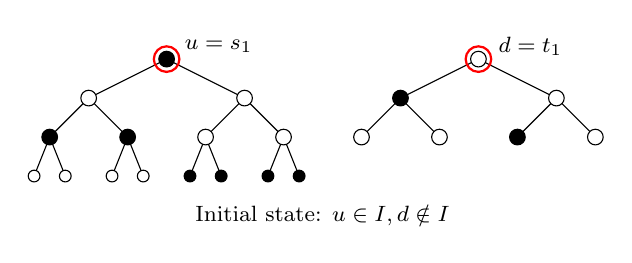
\begin{tikzpicture}[scale=0.33]
    % EDGES
    \draw (-6,-1.5) -- (-9,-3) -- (-10.5,-4.5);
    \draw (-9,-3) -- (-7.5,-4.5);
    \draw (-6,-1.5) -- (-3,-3) -- (-4.5,-4.5);
    \draw (-3,-3) -- (-1.5,-4.5);
    \draw (6,-1.5) -- (3,-3) -- (1.5,-4.5);
    \draw (3,-3) -- (4.5,-4.5);
    \draw (6,-1.5) -- (9,-3) -- (7.5,-4.5);
    \draw (9,-3) -- (10.5,-4.5);
    \foreach \x in {-10.5,-7.5,-4.5,-1.5} {
        \draw (\x,-4.5) -- (\x-0.6,-6);
        \draw (\x,-4.5) -- (\x+0.6,-6);
    }

    % NODES
    %\draw (0,0) node[circle,fill=white,draw,inner sep=2pt] {}; % Root

    % Level 1: 1 Black (u)
    \draw (-6,-1.5) node(u)[circle,fill=black,draw,inner sep=2pt] {};
    \draw (6,-1.5) node(d)[circle,fill=white,draw,inner sep=2pt] {};
    \draw (-4,-1) node[draw=none,fill=none] {\footnotesize $u=s_1$};
    \draw (8,-1) node[draw=none,fill=none] {\footnotesize $d=t_1$};

    % Level 2: 1 Black (dL)
    \draw (-9,-3) node[circle,fill=white,draw,inner sep=2pt] {};
    \draw (-3,-3) node[circle,fill=white,draw,inner sep=2pt] {};
    \draw (3,-3) node[circle,fill=black,draw,inner sep=2pt] {}; % dL
    \draw (9,-3) node[circle,fill=white,draw,inner sep=2pt] {};

    % Level 3: 3 Black (uLL, uLR, dRL)
    \draw (-10.5,-4.5) node[circle,fill=black,draw,inner sep=2pt] {}; % uLL
    \draw (-7.5,-4.5) node[circle,fill=black,draw,inner sep=2pt] {};  % uLR
    \draw (-4.5,-4.5) node[circle,fill=white,draw,inner sep=2pt] {};
    \draw (-1.5,-4.5) node[circle,fill=white,draw,inner sep=2pt] {};
    \draw (1.5,-4.5) node[circle,fill=white,draw,inner sep=2pt] {};
    \draw (4.5,-4.5) node[circle,fill=white,draw,inner sep=2pt] {};
    \draw (7.5,-4.5) node[circle,fill=black,draw,inner sep=2pt] {};   % dRL
    \draw (10.5,-4.5) node[circle,fill=white,draw,inner sep=2pt] {};

    % Level 4: 6 Black
    % uLL, uLR (Black) -> Children White
    \foreach \x in {-11.1,-9.9,-8.1,-6.9} \draw (\x,-6) node[circle,fill=white,draw,inner sep=1.5pt] {};
    % uRL (White) -> Children Black (2)
    \draw (-5.1,-6) node[circle,fill=black,draw,inner sep=1.5pt] {};
    \draw (-3.9,-6) node[circle,fill=black,draw,inner sep=1.5pt] {};
    % uRR (White) -> Children Black (2)
    \draw (-2.1,-6) node[circle,fill=black,draw,inner sep=1.5pt] {};
    \draw (-0.9,-6) node[circle,fill=black,draw,inner sep=1.5pt] {};
    % dLL, dLR (White) -> Children White (Safe)
    %\foreach \x in {0.9, 2.1, 3.9, 5.1} \draw (\x,-6) node[circle,fill=white,draw,inner sep=1.5pt] {};
    % dRL (Black) -> Children White
    %\foreach \x in {6.9, 8.1} \draw (\x,-6) node[circle,fill=white,draw,inner sep=1.5pt] {};
    % dRR (White) -> Children Black (2)
    %\draw (9.9,-6) node[circle,fill=black,draw,inner sep=1.5pt] {};
    %\draw (11.1,-6) node[circle,fill=black,draw,inner sep=1.5pt] {};

    
    % Highlights
    \draw[red, thick] (u) circle (14pt);
    \draw[red, thick] (d) circle (14pt);
    
    \node at (0, -7.5) {\footnotesize Initial state: $u \in I, d \notin I$};
\end{tikzpicture}

\cr

$\xrightarrow[\mbox{    }s_1 \to t_1\mbox{    }]{\mbox{    }\text{1st iteration} \mbox{    }}$ &

% --- STEP 1 STATE ---
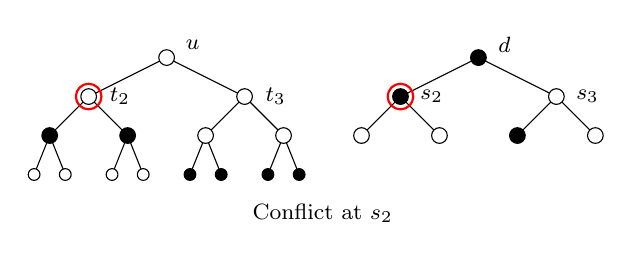
\begin{tikzpicture}[scale=0.33]
    % EDGES
    \draw (-6,-1.5) -- (-9,-3) -- (-10.5,-4.5);
    \draw (-9,-3) -- (-7.5,-4.5);
    \draw (-6,-1.5) -- (-3,-3) -- (-4.5,-4.5);
    \draw (-3,-3) -- (-1.5,-4.5);
    \draw (6,-1.5) -- (3,-3) -- (1.5,-4.5);
    \draw (3,-3) -- (4.5,-4.5);
    \draw (6,-1.5) -- (9,-3) -- (7.5,-4.5);
    \draw (9,-3) -- (10.5,-4.5);
    \foreach \x in {-10.5,-7.5,-4.5,-1.5} {
        \draw (\x,-4.5) -- (\x-0.6,-6);
        \draw (\x,-4.5) -- (\x+0.6,-6);
    }

    % NODES
    %\draw (0,0) node[circle,fill=white,draw,inner sep=2pt] {};

    % Level 1: SWAPPED
    \draw (-6,-1.5) node[circle,fill=white,draw,inner sep=2pt] {}; % u Out
    \draw (6,-1.5) node[circle,fill=black,draw,inner sep=2pt] {};  % d In
    \draw (-5,-1) node[draw=none,fill=none] {\footnotesize $u$};
    \draw (7,-1) node[draw=none,fill=none] {\footnotesize $d$};

    % Level 2: Conflict at dL
    \draw (-9,-3) node(uL)[circle,fill=white,draw,inner sep=2pt] {}; % Target
    \draw (-3,-3) node[circle,fill=white,draw,inner sep=2pt] {};
    \draw (3,-3) node(dL)[circle,fill=black,draw,inner sep=2pt] {};  % Source (Conflict)
    \draw (9,-3) node[circle,fill=white,draw,inner sep=2pt] {};
    \draw (4.2,-3) node[draw=none,fill=none] {\footnotesize $s_2$};
    \draw (10.2,-3) node[draw=none,fill=none] {\footnotesize $s_3$};
    \draw (-1.8,-3) node[draw=none,fill=none] {\footnotesize $t_3$};
    \draw (-7.8,-3) node[draw=none,fill=none] {\footnotesize $t_2$};

    % Level 3: Unchanged
    \draw (-10.5,-4.5) node[circle,fill=black,draw,inner sep=2pt] {};
    \draw (-7.5,-4.5) node[circle,fill=black,draw,inner sep=2pt] {};
    \draw (-4.5,-4.5) node[circle,fill=white,draw,inner sep=2pt] {};
    \draw (-1.5,-4.5) node[circle,fill=white,draw,inner sep=2pt] {};
    \draw (1.5,-4.5) node[circle,fill=white,draw,inner sep=2pt] {};
    \draw (4.5,-4.5) node[circle,fill=white,draw,inner sep=2pt] {};
    \draw (7.5,-4.5) node[circle,fill=black,draw,inner sep=2pt] {};
    \draw (10.5,-4.5) node[circle,fill=white,draw,inner sep=2pt] {};

    % Level 4: Unchanged
    \foreach \x in {-11.1,-9.9,-8.1,-6.9} \draw (\x,-6) node[circle,fill=white,draw,inner sep=1.5pt] {};
    \foreach \x in {-5.1,-3.9,-2.1,-0.9} \draw (\x,-6) node[circle,fill=black,draw,inner sep=1.5pt] {};
    %\foreach \x in {0.9, 2.1, 3.9, 5.1} \draw (\x,-6) node[circle,fill=white,draw,inner sep=1.5pt] {};
    %\foreach \x in {6.9, 8.1} \draw (\x,-6) node[circle,fill=white,draw,inner sep=1.5pt] {};
    %\foreach \x in {9.9, 11.1} \draw (\x,-6) node[circle,fill=black,draw,inner sep=1.5pt] {};

    % Highlights
    \draw[red, thick] (uL) circle (14pt);
    \draw[red, thick] (dL) circle (14pt);
    
    \node at (0, -7.5) {\footnotesize Conflict at $s_2$};
\end{tikzpicture} \\

% =========================================================
% ROW 2: Step 2 -> Step 3
% =========================================================

$\xrightarrow[\mbox{    }s_2 \to t_2\mbox{    }]{\mbox{    }\text{2nd and 3rd iterations}\mbox{    }}$ &

% --- STEP 2 STATE ---
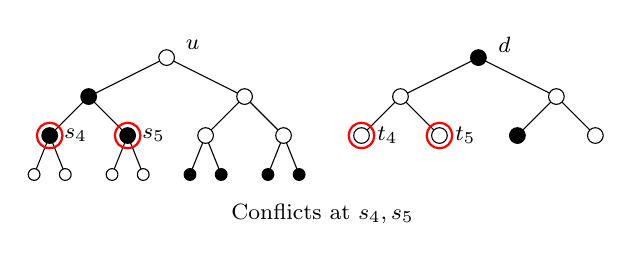
\begin{tikzpicture}[scale=0.33]
    % EDGES
    \draw (-6,-1.5) -- (-9,-3) -- (-10.5,-4.5);
    \draw (-9,-3) -- (-7.5,-4.5);
    \draw (-6,-1.5) -- (-3,-3) -- (-4.5,-4.5);
    \draw (-3,-3) -- (-1.5,-4.5);
    \draw (6,-1.5) -- (3,-3) -- (1.5,-4.5);
    \draw (3,-3) -- (4.5,-4.5);
    \draw (6,-1.5) -- (9,-3) -- (7.5,-4.5);
    \draw (9,-3) -- (10.5,-4.5);
    \foreach \x in {-10.5,-7.5,-4.5,-1.5} {
        \draw (\x,-4.5) -- (\x-0.6,-6);
        \draw (\x,-4.5) -- (\x+0.6,-6);
    }

    % NODES
    %\draw (0,0) node[circle,fill=white,draw,inner sep=2pt] {};
    \draw (-6,-1.5) node[circle,fill=white,draw,inner sep=2pt] {}; 
    \draw (6,-1.5) node[circle,fill=black,draw,inner sep=2pt] {}; 
    \draw (-5,-1) node[draw=none,fill=none] {\footnotesize $u$};
    \draw (7,-1) node[draw=none,fill=none] {\footnotesize $d$};
    
    % Level 2: SWAPPED
    \draw (-9,-3) node[circle,fill=black,draw,inner sep=2pt] {};  % uL In
    \draw (-3,-3) node[circle,fill=white,draw,inner sep=2pt] {};
    \draw (3,-3) node[circle,fill=white,draw,inner sep=2pt] {};   % dL Out
    \draw (9,-3) node[circle,fill=white,draw,inner sep=2pt] {};

    % Level 3: Conflict at uLL, uLR
    \draw (-10.5,-4.5) node(uLL)[circle,fill=black,draw,inner sep=2pt] {}; % Source
    \draw (-7.5,-4.5) node(uLR)[circle,fill=black,draw,inner sep=2pt] {};  % Source
    \draw (-4.5,-4.5) node[circle,fill=white,draw,inner sep=2pt] {};
    \draw (-1.5,-4.5) node[circle,fill=white,draw,inner sep=2pt] {};
    \draw (1.5,-4.5) node(dLL)[circle,fill=white,draw,inner sep=2pt] {};   % Target
    \draw (4.5,-4.5) node(dLR)[circle,fill=white,draw,inner sep=2pt] {};   % Target
    \draw (7.5,-4.5) node[circle,fill=black,draw,inner sep=2pt] {};
    \draw (10.5,-4.5) node[circle,fill=white,draw,inner sep=2pt] {};
    \draw (-9.5,-4.5) node[draw=none,fill=none] {\footnotesize $s_4$};
    \draw (-6.5,-4.5) node[draw=none,fill=none] {\footnotesize $s_5$};
    %\draw (-3.5,-4.5) node[draw=none,fill=none] {\footnotesize $s_6$};
    %\draw (-0.5,-4.5) node[draw=none,fill=none] {\footnotesize $s_7$};
    \draw (2.5,-4.5) node[draw=none,fill=none] {\footnotesize $t_4$};
    \draw (5.5,-4.5) node[draw=none,fill=none] {\footnotesize $t_5$};
    %\draw (8.5,-4.5) node[draw=none,fill=none] {\footnotesize $t_6$};
    %\draw (11.5,-4.5) node[draw=none,fill=none] {\footnotesize $t_7$};
    
    % Level 4: Unchanged
    \foreach \x in {-11.1,-9.9,-8.1,-6.9} \draw (\x,-6) node[circle,fill=white,draw,inner sep=1.5pt] {};
    \foreach \x in {-5.1,-3.9,-2.1,-0.9} \draw (\x,-6) node[circle,fill=black,draw,inner sep=1.5pt] {};
    %\foreach \x in {0.9, 2.1, 3.9, 5.1} \draw (\x,-6) node[circle,fill=white,draw,inner sep=1.5pt] {};
    %\foreach \x in {6.9, 8.1} \draw (\x,-6) node[circle,fill=white,draw,inner sep=1.5pt] {};
    %\foreach \x in {9.9, 11.1} \draw (\x,-6) node[circle,fill=black,draw,inner sep=1.5pt] {};
    

    % Highlights
    \draw[red, thick] (uLL) circle (14pt); \draw[red, thick] (uLR) circle (14pt);
    \draw[red, thick] (dLL) circle (14pt); \draw[red, thick] (dLR) circle (14pt);

    \node at (0, -7.5) {\footnotesize Conflicts at $s_4, s_5$};
\end{tikzpicture}

\cr

$\xrightarrow[\mbox{    }s_4 \to t_4,\ s_5\to t_5\mbox{    }]{\mbox{    }\text{4th and 5th iterations}\mbox{    }}$ &

% --- STEP 3 STATE ---
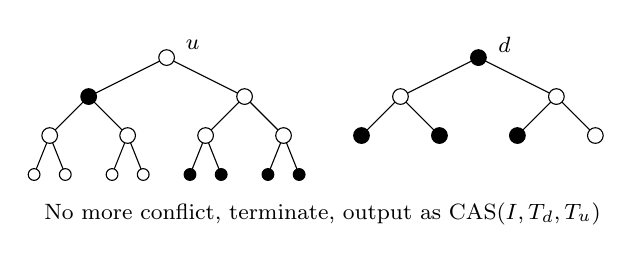
\begin{tikzpicture}[scale=0.33]
    % EDGES
    \draw (-6,-1.5) -- (-9,-3) -- (-10.5,-4.5);
    \draw (-9,-3) -- (-7.5,-4.5);
    \draw (-6,-1.5) -- (-3,-3) -- (-4.5,-4.5);
    \draw (-3,-3) -- (-1.5,-4.5);
    \draw (6,-1.5) -- (3,-3) -- (1.5,-4.5);
    \draw (3,-3) -- (4.5,-4.5);
    \draw (6,-1.5) -- (9,-3) -- (7.5,-4.5);
    \draw (9,-3) -- (10.5,-4.5);
    \foreach \x in {-10.5,-7.5,-4.5,-1.5} {
        \draw (\x,-4.5) -- (\x-0.6,-6);
        \draw (\x,-4.5) -- (\x+0.6,-6);
    }

    \draw (-5,-1) node[draw=none,fill=none] {\footnotesize $u$};
    \draw (7,-1) node[draw=none,fill=none] {\footnotesize $d$};
    % NODES
    %\draw (0,0) node[circle,fill=white,draw,inner sep=2pt] {};
    \draw (-6,-1.5) node[circle,fill=white,draw,inner sep=2pt] {}; 
    \draw (6,-1.5) node[circle,fill=black,draw,inner sep=2pt] {}; 
    \draw (-9,-3) node[circle,fill=black,draw,inner sep=2pt] {}; 
    \draw (-3,-3) node[circle,fill=white,draw,inner sep=2pt] {};
    \draw (3,-3) node[circle,fill=white,draw,inner sep=2pt] {}; 
    \draw (9,-3) node[circle,fill=white,draw,inner sep=2pt] {};

    % Level 3: SWAPPED
    \draw (-10.5,-4.5) node[circle,fill=white,draw,inner sep=2pt] {}; % Out
    \draw (-7.5,-4.5) node[circle,fill=white,draw,inner sep=2pt] {};  % Out
    \draw (-4.5,-4.5) node[circle,fill=white,draw,inner sep=2pt] {};
    \draw (-1.5,-4.5) node[circle,fill=white,draw,inner sep=2pt] {};
    \draw (1.5,-4.5) node[circle,fill=black,draw,inner sep=2pt] {};   % In
    \draw (4.5,-4.5) node[circle,fill=black,draw,inner sep=2pt] {};   % In
    \draw (7.5,-4.5) node[circle,fill=black,draw,inner sep=2pt] {};
    \draw (10.5,-4.5) node[circle,fill=white,draw,inner sep=2pt] {};

    % Level 4: Valid Check
    % Children of dLL, dLR (now Black) MUST be White.
    % In initial setup, they were White.
    %\foreach \x in {0.9, 2.1, 3.9, 5.1} \draw (\x,-6) node[circle,fill=white,draw,inner sep=1.5pt] {};
    
    % Rest of L4
    \foreach \x in {-11.1,-9.9,-8.1,-6.9} \draw (\x,-6) node[circle,fill=white,draw,inner sep=1.5pt] {};
    \foreach \x in {-5.1,-3.9,-2.1,-0.9} \draw (\x,-6) node[circle,fill=black,draw,inner sep=1.5pt] {};
    %\foreach \x in {6.9, 8.1} \draw (\x,-6) node[circle,fill=white,draw,inner sep=1.5pt] {};
    %\foreach \x in {9.9, 11.1} \draw (\x,-6) node[circle,fill=black,draw,inner sep=1.5pt] {};
    
    \node at (0, -7.5) {\footnotesize No more conflict, terminate, output as $\cas(I,T_d,T_u)$};
\end{tikzpicture}

\end{tabular}
    \caption{Example run of CAS with $r=2$. Vertices in $I_i$ are black, and vertices to be modified in each step are circled in red.}
    \label{fig:1}
\end{figure}

\begin{comment}
\begin{definition}[Conditional Alternating Swap]\label{def:CAS}
Let $s$ (Source) and $t$ (Target) be roots of isomorphic subtrees. Let $I$ be an independent set. The CAS operation transforms $I$ into $I'$ using two synchronised queues, $Q_{src}$ and $Q_{tgt}$, initialised with $s$ and $t$.
The process proceeds as follows:
\begin{enumerate}
    \item Dequeue $u$ from $Q_{src}$ and $w$ from $Q_{tgt}$.
    \item \textbf{Pruning Condition:} If $u \notin I$, \textbf{continue} (terminate this branch of traversal). The mapping is identity for the subtree rooted at $u$.
    \item \textbf{Swap Action:} If $u \in I$, set $I' \leftarrow (I \setminus \{u\}) \cup \{w\}$.
    \item \textbf{Crossing Expansion:}
    \begin{itemize}
        \item Enqueue children of $u$ into $Q_{tgt}$ (Target Queue).
        \item Enqueue children of $w$ into $Q_{src}$ (Source Queue).
    \end{itemize}
\end{enumerate}
\end{definition}

\textbf{Remark:} The "Crossing Expansion" is the algorithmic realization of the code's propagation logic. Children of the check node ($u$) are pushed to the space queue ($Q_{tgt}$), and children of the space node ($w$) are pushed to the check queue ($Q_{src}$). This creates an alternating dependency that preserves independence.
\end{comment}

The following key lemma shows that the CAS operation is injective.
\begin{lemma}[Injectivity of CAS]\label{lem:injcas}
For $T_d$ and $T_u$ satisfying the assumptions in Definition~\ref{def:CAS}, the map $I\mapsto\cas(I,T_d,T_u)$ is injective. 
\end{lemma}
\begin{proof}
Let $I,I'\subseteq V(T_d)\cup V(T_u)$ be distinct independent sets containing $u$ but not $d$. We want to show that $\cas(I,T_d,T_u)\not=\cas(I',T_d,T_u)$. This is immediate if $|I|\not=|I'|$ as the CAS operation preserves size, so suppose $|I|=|I'|$. 

For each $i\geq 1$, let $I_i$ and $I_i'$ be the sets obtained at the beginning of the $i$-th iteration of the CAS process applied to $I$ and $I'$, respectively. 

Observe that if the CAS process applied to $I$ and the CAS process applied to $I'$ agree in their first $i-1$ iterations, then at the beginning of the $i$-th iteration, both processes have the same queues $Q_i^s$, $Q_i^t$, and so the same $s_i$ and $t_i$. If $Q_i^s$ is empty, then they both terminate, and we deal with this case below. If not, then the outcomes of the $i$-th iterations for $I$ and $I'$ entirely depend on whether $s_i\in I_i$ and whether $s_i\in I_i'$. By~\ref{cas:2}, $s_i$ has not been modified, so this is equivalent to whether $s_i\in I$ and whether $s_i\in I'$. If they agree, then the $i$-th iteration also agree, while if not, then as $s_i$ and $t_i$ are not modified in future iterations, the final outputs $\cas(I,T_d,T_u)$ and $\cas(I',T_d,T_u)$ differ as one of them contains $t_i$ and the other one doesn't. Therefore, the outputs differ if they disagree in some iteration of the process.

If both processes agree in each iteration up until termination, then they must terminate at the same time, say at the beginning of the $i$-th iteration. From the paragraph above, $I$ and $I'$ agree on all vertices that had been in $Q_j^s$ for some $j\in[i]$. They also agree on all vertices that have been in $Q_j^t$ for some $j\in[i]$, as by~\ref{cas:2} and~\ref{cas:4}, these vertices are not in $I$ and not in $I'$. Hence, $I$ and $I'$ agree on $V_i$, the set of vertices that have been in either queue. However, $I$ and $I'$ are distinct, so they disagree on some $x\in(V(T_d)\cup V(T_u))\setminus V_i$. Since only vertices in $V_i$ are modified by this process, $\cas(I,T_d,T_u)\not=\cas(I',T_d,T_u)$ as they also disagree on $x$.
\end{proof}
\begin{comment}
\begin{proof}
We construct the inverse process $\text{CAS}^{-1}$. It initialises queues identically with $S$ and $T$.
At any step checking a pair $(u, w)$, we inspect the \emph{target} node $w$ in the image configuration $I'$.
\begin{enumerate}
    \item \textbf{Case 1 ($w \in I'$):} This implies a swap must have occurred in the forward pass. Thus, $u$ must have been in $I$. The inverse operation sets $w \to 0, u \to 1$ and performs the Crossing Expansion (which matches the forward expansion).
    \item \textbf{Case 2 ($w \notin I'$):} This implies no swap occurred. If $u$ had been in $I$, $w$ would be in $I'$ (assuming $w$ was initially available, proved in Lemma \ref{lem:CAS_indep}). Thus, $u$ was not in $I$. The inverse operation terminates the branch, matching the forward pruning.
\end{enumerate}
Since the decision to prune or expand is uniquely determined by the presence of elements in the set, the execution traces of the forward and inverse algorithms are identical. Thus, the mapping is a bijection between the active regions defined by $I$ and $I'$.
\end{proof}
\end{comment}

\begin{comment}
\begin{lemma}[Independence Preservation]\label{lem:CAS_indep}
Let $I$ be an independent set where $s \in I$ and $t$ is available (neighbors of $t$ are not in $I$). Applying CAS results in a valid independent set $I'$.
\end{lemma}
\begin{proof}
We analyse the conflict resolution level-by-level.
\begin{itemize}
    \item \textbf{Level 0 ($u=s, w=t$):} We remove $s$ and add $t$.
    \textit{Conflict Risk:} $t$ might be adjacent to nodes in $I$.
    \textit{Resolution:} Neighbors of $t$ are its parent (handled by assumption) and its children. The children of $t$ are pushed to $Q_{src}$. They will be processed as "source" nodes in the next level.
    
    \item \textbf{Level 1 ($u' \in children(t), w' \in children(s)$):}
    Here $u'$ comes from $Q_{src}$ (originally children of $t$).
    \textit{Subcase A ($u' \in I$):} $u'$ is removed and $w'$ is added. Removing $u'$ resolves the conflict with $t$ added at Level 0. Adding $w'$ is safe because its parent $s$ was removed at Level 0.
    \textit{Subcase B ($u' \notin I$):} The branch is pruned. Since $u' \notin I$, there is no conflict with $t$. $w'$ is not added, so no conflict with $S$ (which is removed anyway).
\end{itemize}
By induction, at any level, if we add a node $w$, its parent was removed in the previous level. If we remove a node $u$, it resolves the potential conflict with its parent added in the previous level.
\end{proof}
\end{comment}

\subsection{Case 1: $d(v,\ell)$ is even}\label{sec:even}
When $d(v, \ell)$ is even, the iterative process defining the injection $\phi_{\textup{even}}:\mathcal{A}_{v,\ell}\to\mathcal{B}_{v,\ell}$ %(implemented as \texttt{makeEvenMap})
proceeds by a sequence of vertex swaps on the path $P_{v,\ell}$, combined with performing the CAS operation on the relevant adjacent subtrees. More precisely, let $I\in\mathcal{A}_{v,\ell}$, we construct $\phi_{\textup{even}}(I)\in\mathcal{B}_{v,\ell}$ of the same size as follows. 

\medskip

\noindent\textbf{Initialisation:} Set $I_1=(I\setminus\{v\})\cup\{\ell\}$, $d_1=p(\ell)$, and $u_1=c_1(v)$. 

\medskip

\noindent\textbf{Iteration Step:} For every integer $i\geq 1$, we say we are at the beginning of the $i$-th iteration if there exists $I_i$ and $d_1,d_2,\ldots,d_i,u_1,u_2,\ldots,u_i\in P_{v,\ell}$ such that the following conditions hold. In what follows, for every $v\in V(T)$, let $T_v$ be the subtree of $T$ induced by $v$ and all of its descendants in $T$. 
\stepcounter{propcounter}
\begin{enumerate}[label = \textbf{\Alph{propcounter}\arabic{enumi}}]
    \item\label{even:1} For every $j\in[i-1]$, $d_{j+1}=p(p(d_j))$ and $u_{j+1}=c_1(c_1(u_j))$. Moreover, either $d_i=u_i$ or $d_i$ is a descendant of $u_i$. 
    \item\label{even:2} Neither $u_i$ nor $p(u_i)$ is in $I_i$. 
    \item\label{even:3} Only vertices in $\{d_1,d_2,\ldots,d_{i-1},u_1,u_2,\ldots,u_{i-1}\}\cup(\cup_{j=1}^{i-1}\cup_{m=2}^r(V(T_{c_m(u_j)})\cup V(T_{c_m(d_j)})))$ have been modified, and every vertex is modified at most once.
    \item\label{even:4} $I_i$ is an independent set if $d_i\not\in I_i$. If $d_i\in I_i$, then the only edge in $I_i$ is $d_ic_1(d_i)$.
\end{enumerate}
Note that after initialisation,~\ref{even:1}--\ref{even:4} hold for $i=1$, so we can begin the first iteration. 

\begin{enumerate}
    \item\textbf{Primary Check:} If $d_i\not\in I_i$, terminate, and let $\phi_{\textup{even}}(I)=I_i$. Note that $\phi_{\textup{even}}(I)=I_i$ is an independent set by~\ref{even:4}. Otherwise, $d_i\in I_i$, continue. Observe that if $d_i\in I_i$, then by~\ref{even:2}, $d_i\not=u_i$. Also, by~\ref{even:1} and~\ref{even:3}, $d_i\in I_i$ implies that for every $2\leq m\leq r$, $c_m(d_i)$ has not been modified, and is in neither $I$ nor $I_i$.
    \item\textbf{Primary Shift:} Let $I_i'=(I_i\setminus\{d_i\})\cup\{u_i\}$. By~\ref{even:2} and~\ref{even:4}, the only possible edges in $I_i'$ are between $u_i$ and its $r$ children. 
    \item\textbf{Conditional Alternating Swap:} For every $2\leq m\leq r$, if $c_m(u_i)\not\in I_i'$, do nothing. Otherwise, we need to resolve the conflict at $c_m(u_i)$. Let $J_{i,m}=I_i'\cap(V(T_{c_m(d_i)})\cup V(T_{c_m(u_i)}))$. Using $d(v,\ell)$ is even,~\ref{even:1},~\ref{even:3}, and $c_m(d_i)\not\in I_i'$, the assumptions in Definition~\ref{def:CAS} are satisfied, so we can let $J_{i,m}'=\cas(J_{i,m},T_{c_m(d_i)},T_{c_m(u_i)})$, which is an independent set of the same size as $J_{i,m}$ that contains $c_m(d_i)$ but not $c_m(u_i)$. Let $I_i''=(I_i'\setminus(\cup_{m=2}^rJ_{i,m}))\cup(\cup_{m=2}^rJ_{i,m}')$. Then $|I_i''|=|I_i'|=|I|$, and the only possible edge in $I_i''$ is $u_ic_1(u_i)$.
    \item\textbf{Secondary Check:} If $c_1(u_i)\not\in I_i''$, then terminate, and let $\phi_{\textup{even}}(I)=I_i''$, which is an independent set. Otherwise, $c_1(u_i)\in I_i''$, continue, noting that $c_1(u_i)\not=p(d_i)$ as $d_i\in I_i$ implies that $p(d_i)\not\in I_i''$ by~\ref{even:3}.
    \item\textbf{Secondary Shift:} Let $I_{i+1}=(I_i''\setminus\{c_1(u_i)\})\cup\{p(d_i)\}$. Let $d_{i+1}=p(p(d_i))$ and $u_{i+1}=c_1(c_1(u_i))$, noting that $d_{i+1}$ is either equal to or a descendant of $u_{i+1}$ as $c_1(u_i)\not=p(d_i)$. Since $c_1(u_i)\in I_i''$, $u_{i+1}=c_1(c_1(u_i))$ is not in $I_{i+1}$ by~\ref{even:3}. It follows that~\ref{even:1}--\ref{even:4} hold with $i+1$ in place of $i$, so we can advance to the $(i+1)$-th iteration.
\end{enumerate}

\noindent\textbf{Termination:} Note that each iteration, if not terminated, reduces the distance between $u_i$ and $d_i$ by 4, so the process must terminate. From above, the output $\phi_{\textup{even}}(I)$ is in $\mathcal{B}_{v,\ell}$. 

\medskip

Similar to Lemma~\ref{lem:injcas}, we now show that $\phi_{\textup{even}}$ is injective.
\begin{lemma}\label{lem:injeven}
If $d(v,\ell)$ is even, then $\phi_{\textup{even}}:\mathcal{A}_{v,\ell}\to\mathcal{B}_{v,\ell}$ is injective. 
\end{lemma}
\begin{proof}
Let $I,\overline{I}\in\mathcal{A}_{v,\ell}$ be distinct, we need to show that $\phi_{\textup{even}}(I)\not=\phi_{\textup{even}}(\overline{I})$. This is immediate if $|I|\not=|\overline{I}|$ as $\phi_{\textup{even}}$ preserves size, so suppose $|I|=|\overline{I}|$.

If $I$ and $\overline{I}$ agree in every iteration of the process above, then the set of vertices that are modified in this process are the same for $I$ and $\overline{I}$. Let this set be $V$, then $I$ and $\overline{I}$ agree on $V$. Since $I\not=\overline{I}$, there exists $x\not\in V$ such that one of $I$ and $\overline{I}$ contains $x$, and the other does not. But since $x\not\in V$, $x$ is not modified by the process, so $\phi_{\textup{even}}(I)\not=\phi_{\textup{even}}(\overline{I})$ as they disagree on $x$.

Otherwise, let $i$ be minimal such that the above process for $I$ and $\overline{I}$ first disagree in the $i$-th iteration. Let $I_i$ and $\overline{I_i}$ be the sets in the beginning of the $i$-th iteration of the process for $I$ and $\overline{I}$, respectively. 

If $I$ and $\overline{I}$ disagree on $d_i$, then so do $I_i$ and $\overline{I_i}$ by~\ref{even:3}. From the Primary Check and Primary Shift steps and using~\ref{even:3}, $\phi_{\textup{even}}(I)\not=\phi_{\textup{even}}(\overline{I})$ as exactly one of them contains $u_i$. If $I$ and $\overline{I}$, and thus $I_i$ and $\overline{I_i}$ agree on $d_i$, then the Primary Check and Primary Shift steps are identical.

If $I_i'$ and $\overline{I_i}'$ disagree on $c_m(u_i)$ for some $2\leq m\leq r$, then the CAS step results in a disagreement between $\phi_{\textup{even}}(I)$ and $\phi_{\textup{even}}(\overline{I})$ on $c_m(d_i)$. Now suppose $I_i'$ and $\overline{I_i}'$ agree on $c_m(u_i)$ for all $2\leq m\leq r$. If $J_{i,m}$ and $\overline{J_{i,m}}$ differ for any $2\leq m\leq r$, then~\ref{even:3} and the injectivity of the CAS operation from Lemma~\ref{lem:injcas} imply that $\phi_{\textup{even}}(I)$ and $\phi_{\textup{even}}(\overline{I})$ differ. Otherwise, the CAS step is identical as well. 

Finally, if $I_i''$ and $\overline{I_i}''$ agree on $c_1(u_i)$, then the Secondary Check and Secondary Shift steps are identical, a contradiction to $I$ and $\overline I$ differing in the $i$-th iteration. If they disagree on $c_1(u_i)$ instead, then $\phi_{\textup{even}}(I)\not=\phi_{\textup{even}}(\overline I)$ as exactly one of them contains $p(d_i)$, completing the proof.
\end{proof}

\begin{comment}
\subsection{Case 1: Even Distance $d(v,\ell)$}

When $d(v,\ell)$ is even, the mapping $\phi_{\textup{even}}$ (implemented as \texttt{makeEvenMap}) proceeds by a sequence of shifts along the path $P_{v,\ell}$, combined with the Configuration Move operation on adjacent subtrees.

Let $I \in \mathcal{A}_{v,\ell}$. We construct $I' = \phi_{\textup{even}}(I)$.

\textbf{Algorithm Description ($\phi_{\textup{even}}$):}

\begin{enumerate}
    \item \textbf{Initialization:} Set $I' = (I \setminus \{v\}) \cup \{l\}$.
    \item \textbf{Pointer Setup:} Initialise two pointers traversing the path $P_{v,\ell}$.
    \begin{itemize}
        \item $u_{down} = p(l)$ (initialised near $l$, moving towards $v$).
        \item $u_{up} = L(v)$ (initialised near $v$, moving towards $l$).
    \end{itemize}
    \item \textbf{Iterative Process:} Start loop:
    \begin{enumerate}
        \item \textbf{Primary Check:} If $u_{down} \notin I'$, terminate. (The potential conflict introduced by adding $l$ is resolved).
        \item \textbf{Primary Shift:} $I' \leftarrow (I' \setminus \{u_{down}\}) \cup \{u_{up}\}$. We move the membership from the lower part of the path to the upper part. Since $v \in I$, $L(v) \notin I$, so $u_{up}$ was initially available, because originally $l$ was in the independent set.
        \item \textbf{Alternating swap:} Let $T_{down}^R$ be the subtree rooted at $R(u_{down})$ and $T_{up}^R$ be the subtree rooted at $R(u_{up})$. Apply CAS($T_{up}^R, T_{down}^R$). Since $u_{up}$ is now in $I'$, $T_{up}^R$ must be empty of elements from $I'$, ensuring the move is valid.
        \item \textbf{Secondary Check:} Let $u_{L, up} = L(u_{up})$. If $u_{L, up} \notin I'$, terminate. (This checks for conflicts generated by the Primary Shift).
        \item \textbf{Secondary Shift:} $I' \leftarrow (I' \setminus \{u_{L, up}\}) \cup \{p(u_{down})\}$. This resolves the conflict by shifting the membership upwards along the path.
        \item \textbf{Advance Pointers:} Move both pointers two steps along the path: $u_{up} \leftarrow L(u_{L, up})$ and $u_{down} \leftarrow p(p(u_{down}))$.
    \end{enumerate}
\end{enumerate}
In this case the distance $d(v,\ell)$ is even and $v\in I$ and $l \notin I$. The parity condition implies that there exist two vertices $x, y \notin I$. Notice that $u_{down}$ is always at the odd distance from $l$, while $u_{L, up}$ is at the even distance from $l$. Thus there is an iteration of the loop such that either $u_{down} \notin I'$ or $u_{L, up} \notin I'$ and the process ends. 
\end{comment}

\subsection{Case 2: Odd Distance $d(v,\ell)$}\label{sec:odd}
Now suppose $d(v,\ell)$ is odd. Let $I \in \mathcal{A}_{v,\ell}$, we construct $\phi_{\textup{odd}}(I)\in\mathcal{B}_{v,\ell}$ as follows. 

\medskip

\noindent\textbf{Initialisation:} Let $I_1=(I\setminus\{v\})\cup\{\ell\}$. Create two queues $Q_1^s$ and $Q_1^t$, containing just $p(\ell)$ and just $c_2(v)$, respectively. Let $L_1=\{\ell,p(\ell)\}$ and $V_1=\{v,c_2(v)\}$.

\medskip

\noindent\textbf{Iteration Step:}
At the beginning of the $i$-th iteration, we have some $I_i,L_i,V_i\subseteq V(T)$ such that the following conditions hold. 
\stepcounter{propcounter}
\begin{enumerate}[label = \textbf{\Alph{propcounter}\arabic{enumi}}]
    \item\label{odd:1} $|Q_i^s|=|Q_i^t|$ and $|I_{i}|=|I|$.
    \item\label{odd:2} $L_i\cup V_i=(\cup_{j=1}^i(Q_j^s\cup Q_j^t))\cup\{v,\ell\}$ is the set of all vertices in $T$ that have been in either queue, along with $v$ and $\ell$. $T[L_i]$ and $T[V_i]$ are disjoint subtrees of $T$. Every vertex in $Q_i^s\cup Q_i^t$ is a leaf in either $T[L_i]$ or $T[V_i]$, and has not been modified by this process.
    \item\label{odd:3} Every edge between vertices in $I_i$ contains a vertex in $Q_i^s$. For every $x\in Q_i^s$, it has exactly one neighbour in $I_i$, which is either $c_1(x)$ or $p(x)$, and it is $c_1(x)$ if and only if $x$ is in $L_i$ and is on $P_{v,\ell}$.
    \item\label{odd:4} $Q_i^t\cap I_i=\varnothing$. %and $p(x)\not\in I_i$. ?????????
    \item\label{odd:5} The distance between $\ell$ and every vertex in $Q_i^s$ is odd, while the distance between $\ell$ and every vertex in $Q_i^t$ is even. 
    \item\label{odd:6} Suppose $s_i$ and $t_i$ are the oldest element in $Q_i^s$ and $Q_i^t$, respectively, then one of them is in $V_i$ and the other is in $L_i$.%If $s\in V(T_d)$ and $t\in V(T_u)$, then the distance between $s$ and $d$ is the same as the distance between $t$ and $u$, and vice versa. 
\end{enumerate} 
Note that~\ref{odd:1}--\ref{odd:6} hold after initialisation, so the first iteration can be started.
\begin{enumerate}
    \item \textbf{Dequeue:} If $Q_i^s=\varnothing$, terminate, and return $\phi_{\textup{odd}}(I)=I_i$, noting that~\ref{odd:3} implies that $I_i$ is an independent set. Otherwise, by~\ref{odd:1}, $Q_i^t\not=\varnothing$ as well. Let the oldest element in $Q_i^s$ and $Q_i^t$ be $s_i$ and $t_i$, respectively. 
    \item \textbf{Conflict Check:} If $s_i\notin I_i$, let $I_{i+1}=I_i$, $L_{i+1}=L_i$, $V_{i+1}=V_i$, $Q_{i+1}^s=Q_i^s\setminus\{s_i\}$, $Q_{i+1}^t=Q_i^t\setminus\{t_i\}$, and advance to the $(i+1)$-th iteration, noting that~\ref{odd:1}--\ref{odd:6} hold for $i+1$. Otherwise, $s_i\in I_i$, continue with the current iteration.
    \item \textbf{Swap Action:} Let $I_{i+1}=(I_i\setminus \{s_i\}) \cup \{t_i\}$, noting that $t_i\not\in I_i$ by~\ref{odd:4}, so $|I_{i+1}|=|I_i|=|I|$ by~\ref{odd:1}. Since $s_i\in Q_i^s$, it has exactly one neighbour in $I_i$ by~\ref{odd:3}, which is either $c_1(s_i)$ or $p(s_i)$. By~\ref{odd:5}, $s_i$ is not a leaf in $T$, so it has $r$ children. Consider three cases.
    \begin{itemize}
        \item Suppose that the unique neighbour of $s_i$ in $I_i$ is $c_1(s_i)$, then $s_i\in L_i$ and $s_i$ is on $P_{v,\ell}$ by~\ref{odd:3}, and $t_i\in V_i$ by~\ref{odd:6}. Remove $s_i$ from $Q_i^s$ and $t_i$ from $Q_i^t$. If $t_i$ is not a leaf in $T$, then for every $2\leq m\leq r$ in order, add $c_m(t_i)$ to $Q_i^s$ and add $c_m(s_i)$ to $Q_i^t$. Then, note that by~\ref{odd:5} and using $d(v,\ell)$ is odd, we have that $p(s_i) \not= v$. Add $p(s_i)$ to $Q_i^t$ and add $c_1(t_i)$ to $Q_i^s$. If $t_i$ is a leaf in $T$, then do nothing. Let the resulting updated queues be $Q_{i+1}^s$ and $Q_{i+1}^t$.
        \item Suppose $s_i\in L_i$ and the unique neighbour of $s_i$ in $I_i$ is $p(s_i)$, then $t_i\in V_i$ by~\ref{odd:6}. Again, first remove $s_i$ from $Q_i^s$ and $t_i$ from $Q_i^t$. Then, if $t_i$ is not a leaf in $T$, for every $m\in[r]$ in order, add $c_m(s_i)$ to $Q_i^t$, and add $c_m(t_i)$ to $Q_i^s$, otherwise do nothing. Let the resulting updated queues be $Q_{i+1}^s$ and $Q_{i+1}^t$. 
        \item Suppose $s_i\in V_i$, then the unique neighbour of $s_i$ in $I_i$ is $p(s_i)$ by~\ref{odd:3}, and $t_i\in L_i$ by~\ref{odd:6}. Remove $s_i$ from $Q_i^s$ and $t_i$ from $Q_i^t$. If $t_i$ is a leaf in $T$, do nothing else. Otherwise, $t_i$ has $r$ children in $T$. For every $2\leq m\leq r$ in order, add $c_m(t_i)$ to $Q_i^s$ and add $c_m(s_i)$ to $Q_i^t$. Next, if $t_i$ is on $P_{v,\ell}$, then by~\ref{odd:2}, either $p(t_i)\not\in L_i\cup V_i$ or $p(t_i) = v$. If $p(t_i)\not=v$, add $p(t_i)$ to $Q_i^s$ and add $c_1(s_i)$ to $Q_i^t$, while if $p(t_i)=v$, do nothing. If instead $t_i$ is not on $P_{v,\ell}$, then $c_1(t_i)\not\in L_i\cup V_i$ by~\ref{odd:2}, in which case add it to $Q_i^s$ and add $c_1(s_i)$ to $Q_i^t$. Let the resulting updated queues be $Q_{i+1}^s$ and $Q_{i+1}^t$. 
    \end{itemize}
\end{enumerate}
Note that in all cases above,~\ref{odd:2} and~\ref{odd:3} imply that the new entrants to the queues are not in $L_i\cup V_i$. After updating $L_i$ to $L_{i+1}$ and $V_i$ to $V_{i+1}$ by including new elements in both queues appropriately, the $i$-th iteration is complete, with all of~\ref{odd:1}--\ref{odd:6} maintained, so we can advance to the $(i+1)$-th iteration. 

\medskip

\noindent\textbf{Termination:} The process must end as each vertex can only be added to either queue once, and each iteration removes a vertex from each queue, so $Q_i^s$ eventually becomes empty. The output $\phi_{\textup{odd}}(I)$ is in $\mathcal{B}_{v,\ell}$ because it is an independent set by~\ref{odd:3}, and it contains $\ell$ but not $v$ by the initialisation step. 

\medskip

Like before, it is straightforward to show that $\phi_{\textup{odd}}$ is injective. The proof is omitted as it is quite similar to that of Lemma~\ref{lem:injcas} and Lemma~\ref{lem:injeven}. 
\begin{lemma}\label{lem:injodd}
If $d(v,\ell)$ is odd, then $\phi_{\textup{odd}}:\mathcal{A}_{v,\ell}\to\mathcal{B}_{v,\ell}$ is injective. 
\end{lemma}
%\begin{proof}
%Similar to Lemma~\ref{lem:injcas} and Lemma~\ref{lem:injeven}.
%\end{proof}

We can now prove Theorem~\ref{thm:main}. 
\begin{proof}[Proof of Theorem~\ref{thm:main}]
By Lemma~\ref{lem:injeven} and Lemma~\ref{lem:injodd}, $|\mathcal{A}_{v,\ell}|\leq|\mathcal{B}_{v,\ell}|$, so  \[|\mathcal{I}_{T}^{k}(v)| = |\mathcal{A}_{v,\ell}| + |\mathcal{C}_{v,\ell}|\leq|\mathcal{B}_{v,\ell}|+|\mathcal{C}_{v,\ell}|=|\cI_T^k(\ell)|.\qedhere\]
\end{proof}


\begin{comment}
\subsection{Case 2: Odd Distance $d(v,\ell)$}

When $d(v,\ell)$ is odd, the mapping $\phi_{\textup{odd}}$ (implemented as \texttt{makeOddMap}) is defined by a synchronised BFS propagation mechanism that matches conflicts with available spaces.

Let $I \in \mathcal{A}_{v,\ell}$. We construct $I' = \phi_{\textup{odd}}(I)$.

\textbf{Algorithm Description ($\phi_{\textup{odd}}$):}

\begin{enumerate}
    \item \textbf{Initialization:} Set $I' = (I \setminus \{v\}) \cup \{l\}$.
    \item \textbf{BFS Setup:} We use two queues: $Q_{check}$ (for potential conflicts) and $Q_{space}$ (for available space). We maintain a set $V_{visited}$ to guide the propagation boundaries.
    \begin{itemize}
        \item Initialise $V_{visited} = \{v,\ell\}$.
        \item Enqueue $p(l)$ to $Q_{check}$ (potential conflict).
        \item Enqueue $R(v)$ to $Q_{space}$ (available space, since $v \in I \implies R(v) \notin I$).
    \end{itemize}
    \item \textbf{Iterative Shifting (BFS loop):} While $Q_{check}$ is not empty:
    \begin{enumerate}
        \item Dequeue $u_{check}$ and $u_{space}$. Mark them $V_{visited}$.
        \item If $u_{check} \notin I'$, continue (no conflict).
        \item \textbf{Shift:} $I' \leftarrow (I' \setminus \{u_{check}\}) \cup \{u_{space}\}$.
        \item \textbf{Propagation:} Update the queues based on the neighbors of the swapped vertices. The expansion logic ensures a structural correspondence (isomorphism) between the regions being explored.
        \begin{itemize}
            \item \emph{Expand $Q_{space}$ (from $u_{check}$)}: If $p(u_{check}) \in V_{visited}$, enqueue $L(u_{check})$ and $R(u_{check})$ (propagate downwards). Else, enqueue $p(u_{check})$ and $R(u_{check})$ (propagate upwards/sideways).
            \item \emph{Expand $Q_{check}$ (from $u_{space}$)}: If $p(u_{space}) \in V_{visited}$, enqueue children of $u_{space}$ (if they exist). Else, enqueue $p(u_{space})$ and $R(u_{space})$.
        \end{itemize}
    \end{enumerate}
\end{enumerate}
This mapping implements a form of cascading shifts, resolving the initial conflict near $l$ by utilizing the space near $v$, and systematically resolving subsequent conflicts using the synchronised BFS. Notice that $u_{check}$ is always at the odd distance from $l$ and $u_{space}$ is at the even distance from $l$. Because of that the children of $u_{check}$ always exist. Since in the setup the algorithm moved to the right subtree, while $l$ is in the left subtree, we do not come to the situation where we can not enqueue the desired two vertices to the $Q_{space}$. The algorithm ends, because when $u_{space}$ is a leaf, then the algorithm does not add any vertices to the $Q_{check}$ and the size of $Q_{check}$ decreases.
\end{comment}

\begin{comment}
\section{Proofs of Correctness}

We now provide a rigorous analysis of the mappings. The core of the proof lies in formalizing the logic of `mirrorSubtree` and `makeOddMap`, specifically the line `if (!tree[curCheck].isInSet) continue;`. This condition implies that the mapping is not a global isomorphism, but a bijection restricted to the "Active Region" of the independent set. We model this via the "Conditional Alternating Swap".


\subsection{Proof of Case 1: Even Distance ($\phi_{\textup{even}}$)}

The algorithm `makeEvenMap` iterates pointers $u_{down}$ (from $l$) and $u_{up}$ (from $v$).
While $u_{down} \in I$:
1. \textbf{Path Shift:} $u_{down} \to u_{up}$. This moves the "token" up the path.
2. \textbf{Side Correction:} Call CAS on $(R(u_{up}), R(u_{down}))$.
   \textit{Note:} Since $u_{down} \in I$, independence implies $R(u_{down}) \cap I = \emptyset$. Thus, the CAS operation immediately encounters the Pruning Condition and performs no swaps. However, structurally, this step represents the mapping's capability to transfer configurations. Since it acts as the identity on empty sets, injectivity is preserved.
3. \textbf{Secondary Shift:} If $L(u_{up}) \in I$, shift $L(u_{up}) \to p(u_{down})$. This resolves the conflict created by filling $u_{up}$ at step 1.

Since the path shifts are reversible permutations and CAS is injective (Lemma \ref{lem:partial_bijection}), $\phi_{\textup{even}}$ is injective.

\subsection{Proof of Case 2: Odd Distance ($\phi_{\textup{odd}}$)}

The algorithm `makeOddMap` is a direct application of CAS.
Initialise $I' = (I \setminus \{v\}) \cup \{l\}$.
Set $Q_{src} \leftarrow \{p(l)\}$, $Q_{tgt} \leftarrow \{R(v)\}$.

\begin{theorem}
$\phi_{\textup{odd}}$ is a valid injection.
\end{theorem}
\begin{proof}
\textbf{Validity:} We remove $v$ and add $l$. This creates a potential conflict at $(l, p(l))$.
The algorithm calls CAS with source $p(l)$.
- If $p(l) \in I$, it is moved to $R(v)$. This resolves the conflict at $l$.
- $R(v)$ is available because $v$ was removed.
- If this move creates conflicts (children of $R(v)$), the Crossing Expansion ensures they are processed as sources in the next step.
By Lemma \ref{lem:CAS_indep}, the resulting set is independent.

\textbf{Injectivity:}
By Lemma \ref{lem:partial_bijection}, the mapping is a bijection on the configurations defined by the active regions.
\end{proof}
\end{comment}

\begin{comment}
\section{Perfect trees with arity $r$}

In this section, we generalise our results to perfect $r$-ary trees. A \emph{perfect $r$-ary tree} is a rooted tree where every internal node has exactly $r$ children, and all leaves are at the same depth. For a vertex $u$, we denote its children as $c_1(u), c_2(u), \dots, c_r(u)$.

\begin{theorem}\label{thm:rarity}
Let $T$ be a perfect $r$-ary tree with $r \geq 2$. For any integer $k \ge 1$, any vertex $v \in V(T)$, and any leaf $l \in V(T)$, we have $|\mathcal{I}_{T}^{k}(v)| \le |\mathcal{I}_{T}^{k}(l)|$.
\end{theorem}

\begin{proof}
The proof follows the strategy of the binary case. Due to the symmetry of perfect trees, the size of the star centreed at $v$ depends only on its depth. We assume without loss of generality that $l$ is a descendant of $c_1(v)$ and that the path $P_{v,\ell}$ consists entirely of edges connecting a parent to its first child. We construct an injective mapping $\phi_r: \mathcal{A}_{v,\ell} \to \mathcal{B}_{v,\ell}$ by generalizing the algorithms $\phi_{\textup{even}}$ and $\phi_{\textup{odd}}$.

We define the \textbf{Generalised Conditional Alternating Swap (Generalised CAS)}. Let $u$ and $d$ be two vertices on the path $P_{v,\ell}$. In the binary case, a shift along the path required swapping configurations between the single right subtrees $T_{R(u)}$ and $T_{R(d)}$. In the $r$-ary case, we must handle the sets of off-path siblings $S(u) = \{c_2(u), \dots, c_r(u)\}$ and $S(d) = \{c_2(d), \dots, c_r(d)\}$. Since $T$ is perfect, for each $j \in \{2, \dots, r\}$, the subtree rooted at $c_j(u)$ is isomorphic to the subtree rooted at $c_j(d)$. The Generalised CAS applies the binary CAS operation pairwise to these isomorphic subtrees. Specifically, if $I$ is the current independent set, the update is:
\[
\forall j \in \{2, \dots, r\}, \quad I \leftarrow \cas(I, T_{c_j(u)}, T_{c_j(d)}).
\]
Since the subtrees are disjoint, these operations are independent and preserve injectivity.

\textbf{Case 1: $d(v,\ell)$ is even.}
We define the mapping $\phi_{r, \textup{even}}$ analogously to Section~\ref{sec:even}. Let $I \in \mathcal{A}_{v,\ell}$.
\begin{enumerate}
    \item Initialise $I_1 = (I \setminus \{v\}) \cup \{\ell\}$. Maintain pointers $d_i$ (moving up from $p(\ell)$) and $u_i$ (moving down from $c_1(v)$).
    \item Perform the \textbf{Primary Check} and \textbf{Primary Shift} along $P_{v,\ell}$. If $d_i \in I_i$, shift the membership to $u_i$.
    \item Perform the \textbf{Generalised CAS} to swap the configurations of the sibling sets $S(d_i)$ and $S(u_i)$. This resolves the conflicts generated by adding $u_i$ and utilises the space freed by removing $d_i$.
    \item Perform the \textbf{Secondary Check} and \textbf{Secondary Shift} on the path vertices $c_1(u_i)$ and $p(d_i)$.
\end{enumerate}

\textbf{Case 2: $d(v,\ell)$ is odd.}
We define $\phi_{r, \textup{odd}}$ utilizing the synchronised propagation method from Section~\ref{sec:odd}. Initialise $Q_i^s$ with $\{p(\ell)\}$ and $Q_i^t$ with the set of all $r-1$ siblings of $c_1(v)$, i.e., $S(v) = \{c_2(v), \dots, c_r(v)\}$. The BFS propagation matches conflicts from the source to the target. When a node $x$ is processed (removed from the set), all its $r$ children $\{c_1(x), \dots, c_r(x)\}$ are added to the respective queue. Since $r \ge 2$, the capacity of the target queue is sufficient to resolve all potential conflicts, ensuring the mapping is well-defined and injective.
\end{proof}
\end{comment}

\section{Multiple disjoint perfect trees}

In this section, we consider a forest $\mathcal{T}$ consisting of disjoint perfect trees. Note that every independent set in $\mathcal{T}$ is formed by taking the disjoint union of an independent set in each perfect tree within $\mathcal{T}$, and every such disjoint union of independent sets is an independent set in $\mathcal{T}$. Hence, by Theorem~\ref{thm:main}, for every $k\geq 1$, $|\cI_{\mathcal{T}}^k(v)|$ can be maximised by taking $v$ to be a leaf of some perfect tree in $\mathcal{T}$.  %Let $\mathcal{I}_{\mathcal{T}}^{k}(\ell)$ denote the family of independent sets of size $k$ in the forest $\mathcal{T}$ containing the leaf $\ell$.

To prove Theorem~\ref{thm:forest}, we need to determine which perfect tree in $\mathcal{T}$ should the maximising leaves come from. This is done via the following two lemmas. The first one compares the leaves of two perfect trees with different arities. 

\begin{lemma}\label{lemma:differentarity}
Let $\mathcal{T}$ be a forest consisting of disjoint perfect trees. Let $T_1, T_2$ be two perfect trees in $\mathcal{T}$ with arities $r_1$ and $r_2$, respectively, where $r_1 < r_2$. Let $\ell_1$ be a leaf of $T_1$ and $\ell_2$ be a leaf of $T_2$. Then $|\mathcal{I}_{\mathcal{T}}^{k}(\ell_1)| \le |\mathcal{I}_{\mathcal{T}}^{k}(\ell_2)|$.
\end{lemma}
\begin{proof}
By symmetry, we may assume that $\ell_1$ is the leftmost leaf of $T_1$, and $\ell_2$ is the leftmost leaf of $T_2$. Let $\mathcal{A}_{\ell_1,\ell_2}=\{I\in\cI^k_{\mathcal{T}}:\ell_1\in I, \ell_2\not\in I\}$ and $\mathcal{B}_{\ell_1,\ell_2}=\{I\in\cI^k_{\mathcal{T}}:\ell_1\not\in I, \ell_2\in I\}$. Like in Section~\ref{sec:main}, it suffices to construct an injection $\phi: \mathcal{A}_{\ell_1,\ell_2}\to\mathcal{B}_{\ell_1,\ell_2}$. Let $I \in \mathcal{A}_{\ell_1,\ell_2}$.
\begin{enumerate}
    \item\textbf{Leaf Swap:} Set $I_1= (I \setminus \{\ell_1\}) \cup \{\ell_2\}$.
    \item\textbf{Primary Check:} If $p(\ell_2)\not\in I_1$, then $I_1\in\mathcal{B}_{\ell_1,\ell_2}$. In this case, let $\phi(I)=I_1$ and terminate. Otherwise, $p(\ell_2)\in I_1$ and we have a conflict. Set $I_2=(I_1\setminus\{p(\ell_2)\})\cup\{p(\ell_1)\}$ and continue.
    %\item\textbf{Primary Shift:} 
    \item\textbf{Secondary Check:} For each $2\leq i\leq r_1$, if $c_i(p(\ell_1))\in I_2$, then remove it from $I_2$ and replace it with $c_i(p(\ell_2))$, otherwise do nothing. If $p(p(\ell_1))\in I_2$, then remove it and replace it with $c_{r_1+1}(p(\ell_2))$, otherwise do nothing. Note that as $p(\ell_2)\in I_1$, $c_i(p(\ell_2))\not\in I_2$ for every $i\in[r_2]$, and $c_{r_1+1}(p(\ell_2))$ exists as $r_1<r_2$. Let $I_3$ be the resulting set. Observe that $I_3\in\mathcal{B}_{\ell_1,\ell_2}$. Let $\phi(I)=I_3$ and terminate.
    %\item \textbf{Sibling Mapping:} If $p(l_1)$ is added, we must map the configuration of its siblings $S(p(l_1))$ to $S(p(l_2))$. Since $r_1 < r_2$, $|S(p(l_1))| < |S(p(l_2))|$. We map the $j$-th sibling of $p(l_1)$ to the $j$-th sibling of $p(l_2)$.
    %\item \textbf{Space Utilization:} If $p(l_1)$ cannot be added because $p(p(l_1)) \in I$, we utilise the higher arity of $T_2$. Instead of propagating the conflict further up in $T_1$, we map the conflicting vertex to the $(r_1+1)$-th sibling of $l_2$ (or its parent's sibling, depending on the depth). Since $r_1 < r_2$, $T_2$ possesses strictly more branches. Specifically, if $p(p(l_1))$ prevents the addition of $p(l_1)$, we remove $p(p(l_1))$ and add the $(r_1+1)$-th sibling of $p(l_2)$. This vertex is available because $p(l_2)$ was removed in Step 2.
\end{enumerate}
It is clear that $\phi$ is an injection, so $|\mathcal{I}_{\mathcal{T}}^{k}(\ell_1)| \le |\mathcal{I}_{\mathcal{T}}^{k}(\ell_2)|$.
\end{proof}

By Lemma~\ref{lemma:differentarity}, $|\cI_{\mathcal{T}}^k(v)|$ is maximised by the leaves of a perfect tree with the highest arity in $\mathcal{T}$. The next lemma compares leaves in two perfect trees with the same arity. 
\begin{lemma}\label{lemma:samearity}
Let $\mathcal{T}$ be a forest consisting of disjoint perfect trees. Let $T_1, T_2$ be perfect trees in $\mathcal{T}$ with equal arity $r$ containing $h_1$ and $h_2$ levels, respectively, where $h_1 < h_2$. Let $\ell_1 \in V(T_1)$ and $\ell_2 \in V(T_2)$ be leaves.
\begin{itemize}
    \item If $h_1$ is even, then $|\mathcal{I}_{\mathcal{T}}^{k}(\ell_1)| \le |\mathcal{I}_{\mathcal{T}}^{k}(\ell_2)|$.
    \item If $h_1$ is odd, then $|\mathcal{I}_{\mathcal{T}}^{k}(\ell_1)| \ge |\mathcal{I}_{\mathcal{T}}^{k}(\ell_2)|$.
\end{itemize}
\end{lemma}
\begin{proof}
Let $\mathcal{A}_{\ell_1,\ell_2}=\{I\in\cI^k_{\mathcal{T}}:\ell_1\in I, \ell_2\not\in I\}$ and $\mathcal{B}_{\ell_1,\ell_2}=\{I\in\cI^k_{\mathcal{T}}:\ell_1\not\in I, \ell_2\in I\}$. This is very similar to the proofs in Section~\ref{sec:main}, so we will be less formal and omit some details. %We utilise the path parity argument from Section 3.
Let $\varphi:V(T_1)\to V(T_2)$ be an injective homomorphism mapping $\ell_1$ to $\ell_2$. Define $\psi:V(T_1)\cup\varphi(V(T_1))\to V(T_1)\cup\varphi(V(T_1))$ by letting $\psi(v)=\varphi(v)$ if $v\in V(T_1)$, and $\psi(v)=\varphi^{-1}(v)$ if $v\in\varphi(V(T_1))$. In other words, $\psi$ maps every vertex in $V(T_1)\cup\varphi(V(T_1))$ to the corresponding vertex in its counterpart. 

\textbf{Case 1:} $h_1$ is even. We construct an injection $\phi:\mathcal{A}_{\ell_1,\ell_2}\to\mathcal{B}_{\ell_1,\ell_2}$ using the following algorithm. Initialise with $I_1 = (I \setminus \{\ell_1\}) \cup \{\ell_2\}$ and two queues $Q_1^s=\{p(\ell_2)\}$ and $Q_1^t=\{p(\ell_1)\}$. Throughout, we will maintain the key condition that if $v\in Q_i^s$, then $\psi(v)\in Q_i^t$ and $\psi(v)\not\in I_i$. 

In the $i$-th iteration, given $I_i$, $Q_i^s$, and $Q_i^t$, if $Q_i^s=\varnothing$, terminate and return $\phi(I)=I_i$. Otherwise, dequeue the oldest element $s_i$ in $Q_i^s$ and the corresponding element $\psi(s_i)$ in $Q_i^t$. If $s_i\not\in I_i$, advance to the next iteration with $I_{i+1}=I_i$. Otherwise, $s_i\in I_i$. Let $I_{i+1}=(I_i\setminus\{s_i\})\cup\{\psi(s_i)\}$. For each neighbour $v$ of $\psi(s_i)$ that has not been visited, add $v$ to $Q_i^s$ and add $\psi(v)$ to $Q_i^t$. Note that $\psi(v)$ also has not been visited, and since $\psi(v)$ is a neighbour of $s_i$ which is in $I_i$, we have $\psi(v)\not\in I_{i+1}$, so the key condition above is maintained. 

Furthermore, before termination, the vertices on the path $P$ between $p(\ell_1)$ and the root $x_1$ of $T_1$ alternate from being added to $Q_i^t$ and being added to $Q_i^s$, starting with $p(\ell_1)$ being added to $Q_i^t$ in the initialisation. Since $h_1$ is even, either the algorithm terminates before reaching $x_1$, or $x_1$ is added to $Q_i^t$, so vertices outside of $\varphi(V(T_1))$ in $T_2$ are never visited and the algorithm above is well-defined. Similar to the proofs in Section~\ref{sec:main}, the algorithm must terminate and output $\phi(I)\in\mathcal{B}_{\ell_1,\ell_2}$, and $\phi$ is injective. 
%We propagate conflicts up the path $P_{\ell_2}$. If $p(\ell_2) \in I'$, remove it and add $p(\ell_1)$ (if available). We continue alternating swaps. Since $h_1$ is odd, the root of $T_1$ is at an odd distance from $\ell_1$. The propagation sequence along $P_{\ell_1}$ ensures that if the conflict chain reaches the root of $T_1$, the required operation is to add the root to $I'$. As the root has no parent, this is valid. In $T_2$, the corresponding node at height $h_1$ has a parent, but since we map from the restricted geometry of $T_1$ to $T_2$, the termination at the root of $T_1$ implies we do not occupy the parent in $T_2$, avoiding conflicts.

\textbf{Case 2:} $h_1$ is odd. We similarly construct an injection $\phi:\mathcal{B}_{\ell_1,\ell_2} \to \mathcal{A}_{\ell_1,\ell_2}$. Initialise with $I_1 = (I \setminus \{\ell_2\}) \cup \{\ell_1\}$ and two queues $Q_1^s=\{p(\ell_1)\}$ and $Q_1^t=\{p(\ell_2)\}$. Then, we proceed with the algorithm as in Case 1. Since $h_1$ is now odd and $p(\ell_1)$ is added to $Q_1^s$ in the initialisation, either the algorithm terminates before reaching the root $x_1$ of $T_1$, or $x_1$ is added to $Q_i^t$. This again shows that vertices outside of $\varphi(V(T_1))$ in $T_2$ are never visited and the algorithm is well-defined. At termination, it outputs $\phi(I)\in\mathcal{A}_{\ell_1,\ell_2}$, and $\phi$ is injective. 
%the root of $T_1$ is at an even distance from $\ell_1$. If the configuration in $T_2$ requires occupying the node at height $h_1$ (corresponding to the root of $T_1$), $T_1$ accommodates this as the root has no parent to cause a conflict. Thus, the shorter tree $T_1$ can absorb the configurations of the taller tree $T_2$ when the height parity is even.
\end{proof}

We can now put everything together and quickly deduce Theorem~\ref{thm:forest}.
\begin{proof}[Proof of Theorem~\ref{thm:forest}]
By Theorem~\ref{thm:main}, $|\cI_{\mathcal{T}}^k(v)|$ is maximised by the leaves of some perfect tree in $\mathcal{T}$. By Lemma~\ref{lemma:differentarity}, $|\cI_{\mathcal{T}}^k(v)|$ is maximised by a perfect tree with the highest arity in $\mathcal{T}$. Finally, by Lemma~\ref{lemma:samearity}, if every perfect tree with the highest arity in $\mathcal{T}$ has an even number of levels, then a maximising leaf belongs to the one with the highest number of levels, otherwise it belongs to the one with the lowest odd number of levels.
\end{proof}

%\section{Concluding Remarks}


%We have presented a constructive proof that perfect binary trees satisfy the Hurlbert-Kamat (HK) property; that is, the leaves are the vertices contained in the largest number of independent sets of a fixed size $k$. The proof relies on explicit algorithmic injective mappings that utilise the symmetry and recursive structure of perfect binary trees. These mappings employ distinct strategies based on the parity of the distance between the internal vertex and the leaf, utilizing techniques of synchronised BFS traversals and iterative path adjustments combined with configuration transfers between isomorphic subtrees.

%Furthermore, we extended this constructive framework to perfect trees of arbitrary arity $r \ge 2$, demonstrating that the HK property holds universally for this class of graphs via the Generalised Conditional Alternating Swap. 

%Finally, we analyzed the distribution of independent sets in forests of disjoint perfect trees. By constructing injections between leaves of distinct tree components, we established a hierarchy of star sizes based on the topological parameters of the trees. We demonstrated that the size of a leaf-centreed star is monotone with the arity of the tree. Among trees of equal arity, the maximality is determined by the height parity: the global maximum is attained by a leaf in the tree with the \textbf{smallest even height}. In the absence of trees with even height, the maximum is attained by a leaf in the tree with the \textbf{largest odd height}. These results provide a complete characterization of the extremal independent set distributions in forests of perfect trees.



\bibliographystyle{plain}  
\bibliography{reference}


%\bibitem{LM} V. E. Levit, E. Mandrescu. "The structure of $\alpha$-stable graphs." \textit{arXiv preprint math/0307072} (2003).

%\end{thebibliography}

\begin{comment}
\newpage
\appendix
\section{Appendix: C++ Implementation of Mappings}\label{appendix}

The following C++ code implements the logic for the injective mappings described in Section 3. The \texttt{Vertex} structure represents the tree nodes, and the \texttt{isInSet} boolean flag represents the membership in the independent set being transformed.

\begin{lstlisting}[language=C++, caption=Implementation of Injective Mappings]
#include <bits/stdc++.h>

using namespace std;
typedef long long ll;

struct Vertex {
    ll left = -1, right = -1, parent = -1;
    bool isInSet = false;
    bool visited = false;
    ll id = 0;
};

vector<Vertex> tree;

// Implementation of the mapping for Odd distance (phi_odd) - Section 3.3
void makeOddMap(ll from, ll to) {
    // Initialization (Swap v and l)
    tree[from].isInSet = false;
    tree[to].isInSet = true;
    tree[from].visited = true;
    tree[to].visited = true;

    // BFS Setup (Synchronised Traversal)
    queue<ll> toCheck, posSpace;
    toCheck.push(tree[to].parent); // p(l)
    posSpace.push(tree[from].right); // R(v)

    // Iterative Shifting (BFS loop)
    while (!toCheck.empty()) {
        ll curCheck = toCheck.front();
        tree[curCheck].visited = true;
        toCheck.pop();
        ll curSpace = posSpace.front();
        tree[curSpace].visited = true;
        posSpace.pop();

        if (!tree[curCheck].isInSet) continue;

        // Shift
        tree[curCheck].isInSet = false;
        tree[curSpace].isInSet = true;

        // Propagation Logic
        // Expand Q_space (from neighbors of curCheck)
        if (tree[tree[curCheck].parent].visited) {
            // Propagate downwards
            posSpace.push(tree[curCheck].left);
            posSpace.push(tree[curCheck].right);
        } else {
            // Propagate upwards/sideways
            posSpace.push(tree[curCheck].parent);
            posSpace.push(tree[curCheck].right);
        }

        // Expand Q_check (from neighbors of curSpace)
        if (tree[tree[curSpace].parent].visited) {
            // Propagate downwards (if not a leaf)
            if (tree[curSpace].left != -1) {
                toCheck.push(tree[curSpace].left);
                toCheck.push(tree[curSpace].right);
            }
        } else {
            // Propagate upwards/sideways
            toCheck.push(tree[curSpace].parent);
            toCheck.push(tree[curSpace].right);
        }
    }
}

// Helper function: Configuration Move (Section 3.1)
void mirrorSubtree(ll from, ll to) {
    queue<ll> toCheck, posSpace;
    toCheck.push(from);
    posSpace.push(to);
    while (!toCheck.empty()) {
        ll curCheck = toCheck.front();
        toCheck.pop();
        ll curSpace = posSpace.front();
        posSpace.pop();

        if (!tree[curCheck].isInSet) continue;
        tree[curCheck].isInSet = false;
        tree[curSpace].isInSet = true;

        posSpace.push(tree[curCheck].left);
        posSpace.push(tree[curCheck].right);
        if (tree[curSpace].left != -1) {
            toCheck.push(tree[curSpace].left);
            toCheck.push(tree[curSpace].right);
        }
    }
}

// Implementation of the mapping for Even Distance (phi_even) - Section 3.2
void makeEvenMap(ll from, ll to) {
    // Initialization (Swap v and l)
    tree[from].isInSet = false;
    tree[to].isInSet = true;

    // Pointer Setup
    ll curDown = tree[to].parent; // p(l)
    ll curUp = tree[from].left;   // L(v)

    // Iterative Process
    while (true) {
        // Primary Check
        if (!tree[curDown].isInSet) break;

        // Primary Shift
        tree[curDown].isInSet = false;
        tree[curUp].isInSet = true;

        // Configuration Move (Right subtrees)
        mirrorSubtree(tree[curDown].right, tree[curUp].right);

        // Secondary Check
        if (!tree[tree[curUp].left].isInSet) break; // Check L(u_up)

        // Secondary Shift
        tree[tree[curUp].left].isInSet = false;
        tree[tree[curDown].parent].isInSet = true; // Shift to p(u_down)

        // Advance Pointers
        curUp = tree[tree[curUp].left].left;
        curDown = tree[tree[curDown].parent].parent;
    }
}


int main() {
    ll v, leaf;
    makeOddMap(v, leaf);
    makeEvenMap(v, leaf);
}
\end{lstlisting}
\end{comment}
\end{document}
